% 4.2.1: Assessing gradience

\subsubsection{Response distributions}

This is shown in Figure \ref{density}.

\begin{figure}
\centering
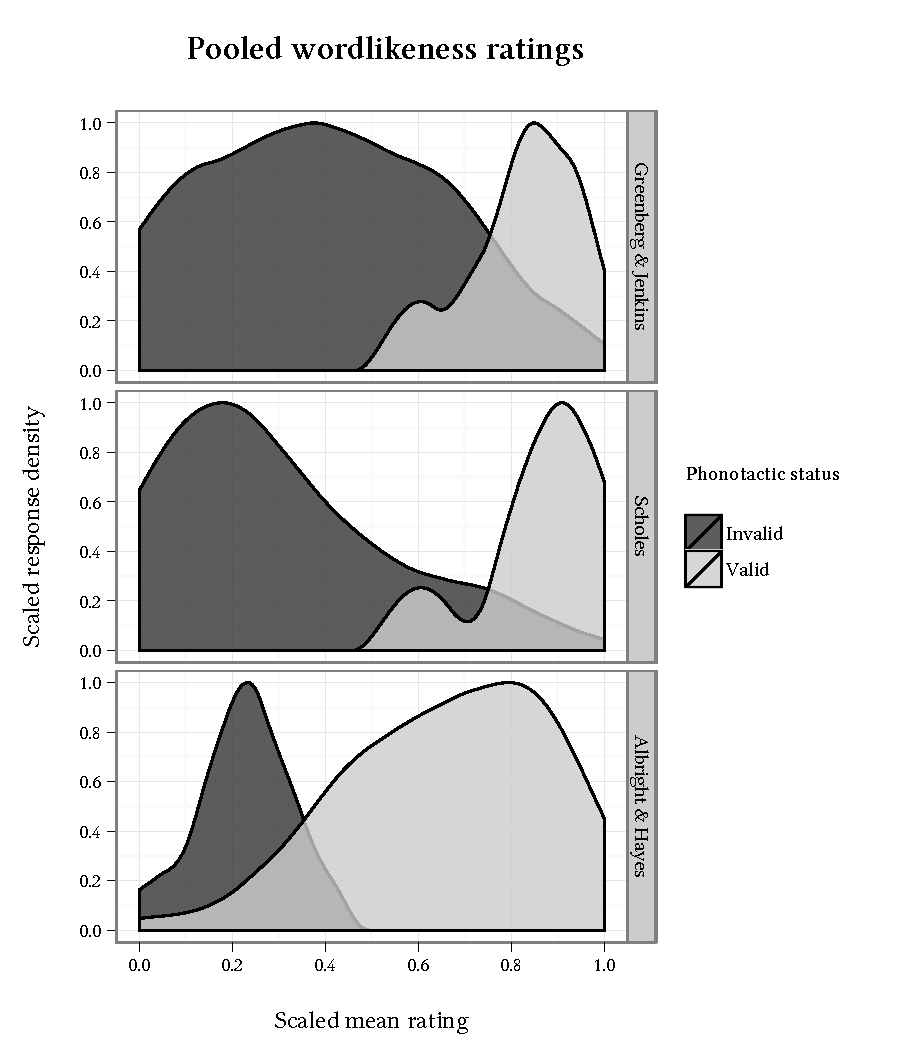
\includegraphics{density.pdf}
\caption{Density of responses}
\label{density}
\end{figure}

\ex EM test results: \vspace{6pt} \\
\begin{tabular}{l | r r | r r r r r r | r r}
\toprule
     & \multicolumn{2}{c|}{one $\mathcal{N}$} & \multicolumn{6}{c|}{mixture of two $\mathcal{N}$s} & \multicolumn{2}{c}{log $\mathcal{L}$ test} \\
     & $\mu$ & $\sigma$ & $\mu_1$ & $\sigma_1$ & mix$_1$ & $\mu_2$ & $\sigma_2$ & mix$_2$ & $\Lambda$ & $p$-value  \\
\midrule
G\&J & 0.378 & 0.295    & 0.150   & 0.090      & 0.436     & 0.554   & 0.278    & 0.564     & 5.190    & 0.158   \\
S    & 0.596 & 0.361    & 0.236   & 0.232      & 0.437     & 0.876   & 0.105    & 0.563 & 48.965    & 1.3\e{-10} \\
A\&H & 0.431 & 0.266    & 0.301   & 0.200      & 0.559     & 0.595   & 0.246    & 0.411 & 16.186    & 0.001      \\
\bottomrule
\end{tabular}
\xe

%\ex Residualized correlations
%\begin{tabular}
%\toprule
%ASDF
%\midrule
%G\&J & 
%S    & 
%A\&H & 
%\bottomrule
%\xe

%\subsubsection{Prediction distributions}

\citet{Coltheart1977}

\citet{Hayes2008a}
\citet{Albright2009a}

% stats thereof
%\citet{Schilling2002}
%\citet{Helguerro1904}
%\citet{Cohen1956}

% EM
\citet{EM}

\footnote{In performing this evaluation, I have benefitted greatly from course notes by Mark Liberman and Stephen Isard.}
%available at \url{http://www.ling.upenn.edu/courses/cogs501/K-meansHW.html}

% -2 log like ratio test

where the difference in degrees o freedom equals $D$

%\ex $\displaystyle \textrm{Reject } H_0 \textrm{ iff } 
%\ex $\displaystyle \Lambda = -2 \textrm{ ln } L_0 + 2 \textrm{ ln } L_1}$ \xe
% > χ^2_{d.f.=D}$ \xe
